\documentclass{article}
\usepackage[utf8]{inputenc}
\usepackage{pgfplots}
\pgfplotsset{width=10cm,compat=1.9}
\usepackage{amsmath,amssymb,amsthm}
\usepackage{gensymb}
\usepackage{graphicx}
\usepackage{amsmath}
\usepackage{float}
\usepackage{enumerate}
\usepackage{xcolor}
\usepackage{blindtext}
\usepackage[margin=1in]{geometry}
\usepackage{hyperref}
\hypersetup{
    colorlinks=true,
    linkcolor=blue,
    filecolor=magenta,      
    urlcolor=cyan,
    pdftitle={Overleaf Example},
    pdfpagemode=FullScreen,
    }
\usepackage[slovene]{babel}

\setlength{\parindent}{0pt}
\setlength{\parskip}{4pt}


\newcounter{example}[section]
\newenvironment{example}[1][]{\refstepcounter{example}\par\medskip
   \noindent \textbf{Naloga~\theexample. #1} \rmfamily}{\medskip}


\title{Vektorji}
\author{Bor Bregant}
\date{\vspace{-5ex}}

\begin{document}

\maketitle

\begin{example}
    V narisanem telesu z označeno bazo izrazi vektorje $\vec{CF'}$ in $\vec{E'X}$, če velja $X\in BB'$, $|BX|:|XB'|=2:1$.
    \begin{figure}[H]
        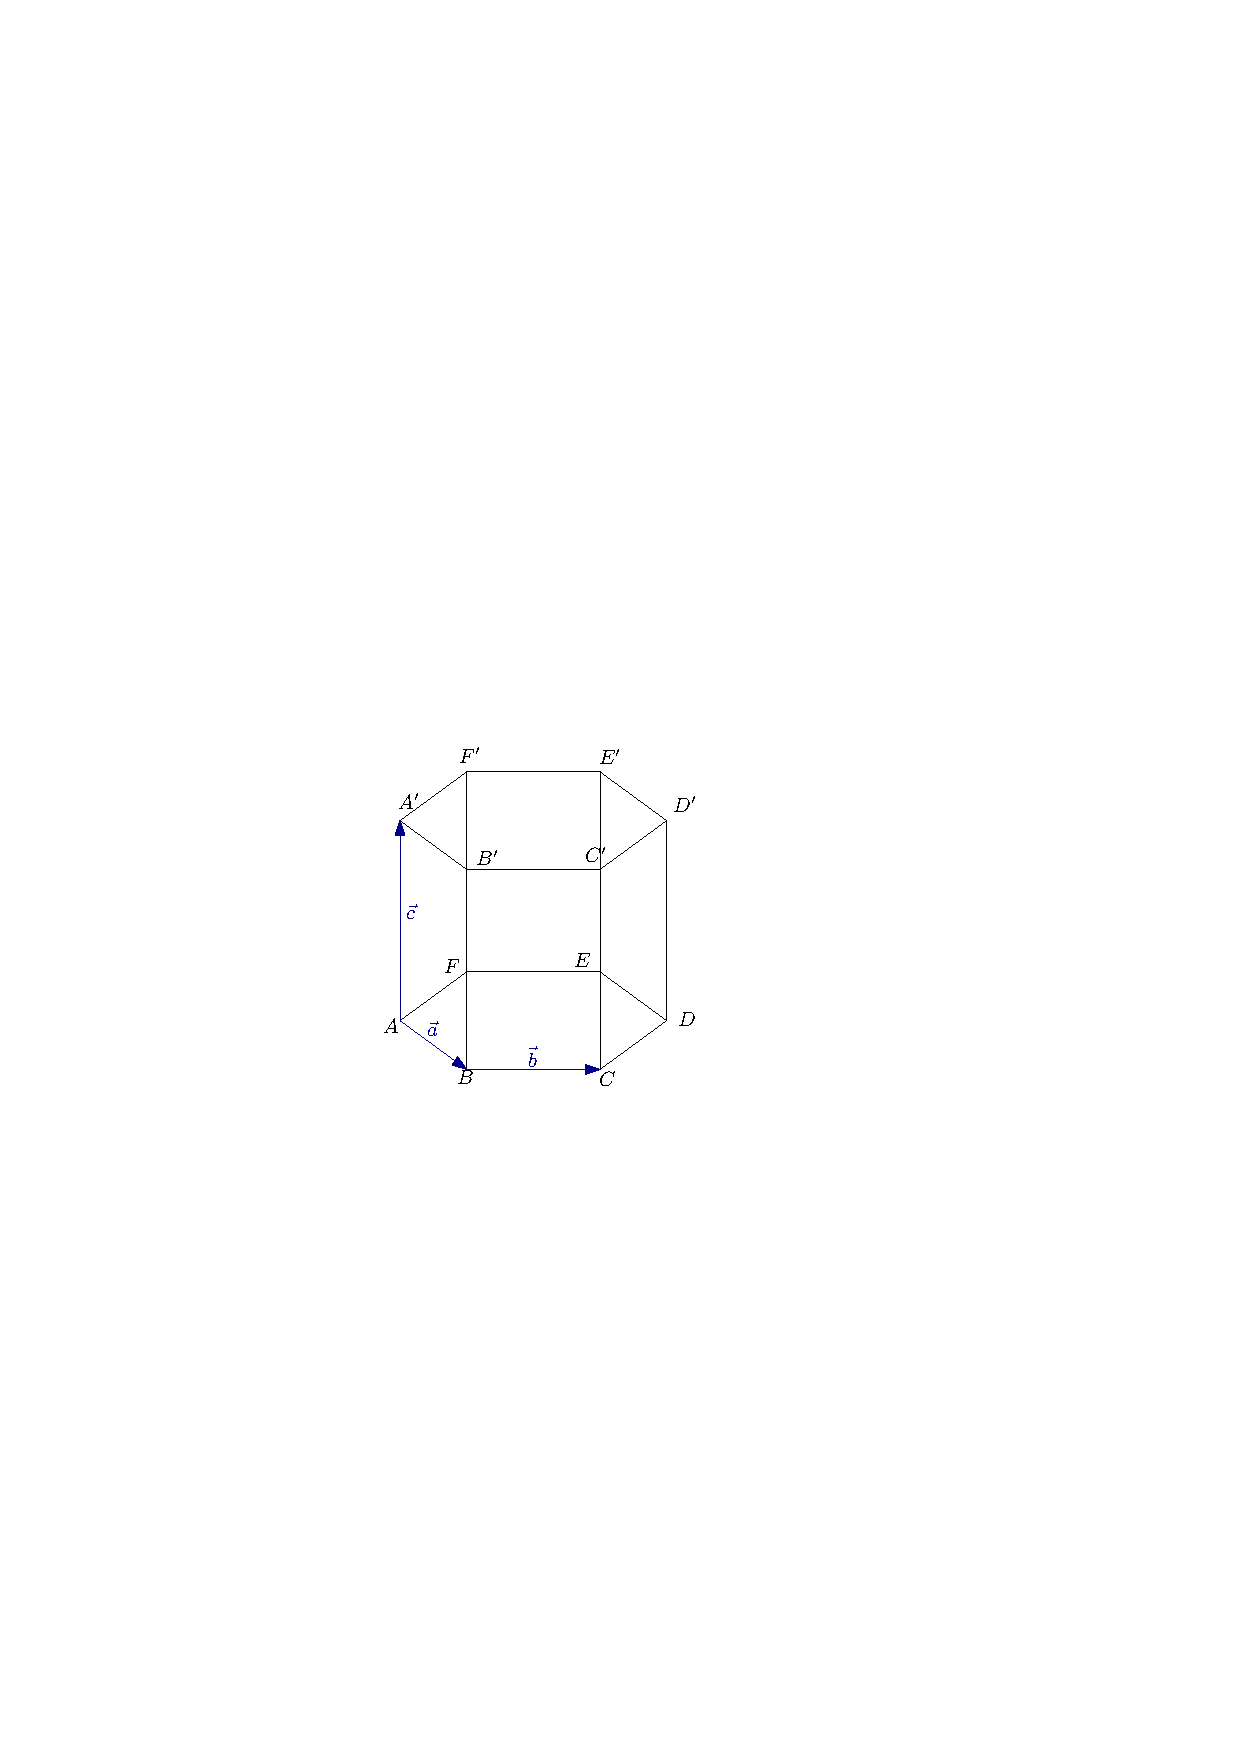
\includegraphics[width=0.35\textwidth]{vektorji_naloga_3d_baza.pdf}
        \centering
    \end{figure}
\end{example}

\begin{example}
    V trikotniku $ABC$ naj je $X\in BC$, $|BX|:|XC|=3:4$ in $Y$ razpolovišče $AC$. V kakšnem razmerju deli $BY$ daljico $AX$.
\end{example}

\begin{example}
    Določi parameter $u$, da bosta vektorja $\vec{a}=(2,-3,\frac{u}{2})$ in $\vec{b}=(-6,9,4)$ kolinearna. Ali so v tem primeru $\vec{a}$, $\vec{b}$ in $\vec{c}=(1,1,1)$ koplanarni?
\end{example}

\begin{example}
    Zapiši formulo za koordinate težišča trikotnika, če imaš podana vsa oglišča.
\end{example}

\begin{example}
    Dolžina vektorja $\vec{a}$ je 8, dolžina vektorja $\vec{b}$ je 5, dolžina $\vec{a}+2\vec{b}$ pa 14. Natančno izračunaj dolžino $\vec{a}-\vec{b}$.
\end{example}

\begin{example}
    V enakokrakem trapezu je $a=8$, $c=4$ in $b=3$. Natančno zračunaj $\alpha$ in $e$.
\end{example}

\begin{example}
    Natančno določi parameter $x$, da vektorja $(5,0)$ in $(2,x)$ oklepala kot $45^\circ$.
\end{example}


\end{document}